%%%%%%%%%%%%%%%%%%%%%%%%%%%%%%%%%%%%%%%%%
% Improvement Of Interpretability In Machine
% Learning Models
%
% Authors:
% Mohammad Ali Kazemi Ardekani
%
% NOTE: The bibliography needs to be compiled using the biber engine.
%%%%%%%%%%%%%%%%%%%%%%%%%%%%%%%%%%%%%%%%%

%----------------------------------------------------------------------------------------
%	PACKAGES AND OTHER DOCUMENT CONFIGURATIONS
%----------------------------------------------------------------------------------------

\documentclass[a4paper, 10pt,]{JournalArticle}

\usepackage{stfloats}

\usepackage[none]{hyphenat}

\usepackage{amsmath,amssymb,amsthm} % For including math equations, theorems, symbols, etc

\addbibresource{references.bib} % BibLaTeX bibliography file

\runninghead{Interpretability of Machine Learning} % A shortened article title to appear in the running head

\setcounter{page}{1} % The page number of the first page

%----------------------------------------------------------------------------------------
%	TITLE SECTION
%----------------------------------------------------------------------------------------

\title{Improvement Of Interpretability \\ In Machine Learning Models} % Article title

\author{
	Mohammad Ali Kazemi Ardekani\textsuperscript{1}
}


\date{\footnotesize\textsuperscript{\textbf{1}}Faculty of Electronics and Computer Engineering, Shiraz University, Shiraz, Iran}

% Full-width abstract
\renewcommand{\maketitlehookd}{
	\begin{abstract}
		\noindent In the realm of machine learning, interpretability stands as a fundamental challenge of considerable significance. With remarkable strides in this field, the need for systems capable of providing accurate and predictable responses has never been more pronounced. This article aims to present innovative solutions and techniques for improving interpretability in machine learning. Sometimes our model has bias due to erroneous assumptions in machine learning process that we could resolve it by analyzing our model using interpretability methods. \\ \\
  \normalfont{
    \textbf{Keywords:} \keyword{Machine Learning, Interpretability, Bias, Interpretability Methods, LIME, SHAP, Anchors}
}
	\end{abstract}
}

%----------------------------------------------------------------------------------------

\begin{document}

\maketitle
%----------------------------------------------------------------------------------------
%	ARTICLE CONTENTS
%----------------------------------------------------------------------------------------
\section{Introduction}

Machine learning is a subset of artificial intelligence that enables computers to learn and improve performance on specific tasks without explicit programming. It encompasses supervised learning, where algorithms are trained on labeled data; unsupervised learning, which discovers patterns in unlabeled data; and reinforcement learning, involving agents interacting with environments to optimize rewards. The success of machine learning models depends on factors like data quality and algorithm choice. Interpretability, or the seamless integration of different systems and tools, plays a crucial role in maximizing the effectiveness of machine learning applications, ensuring they can collaborate with diverse technologies and datasets to deliver robust and adaptable solutions across various domains. \cite{mitchell1997machine}

%------------------------------------------------

\section{Interpretability}
\textbf{Interpretability is the degree to which a human can understand the cause of a decision.} \cite{miller2019explanation}

The higher the interpretability of a machine learning model, the easier it is for someone to comprehend why certain decisions or predictions have been made. A model is better interpretable than another model if its decisions are easier for a human to comprehend than decisions from the other model.

Interpretable machine learning is a useful umbrella term that captures the “extraction of relevant knowledge from a machine-learning model concerning relationships either contained in data or learned by the model”.

%------------------------------------------------

\section{Evaluation of Interpretability}

There is no real consensus about what interpretability is in machine learning. Nor is it clear how to measure it. But there is some initial research on this and an attempt to formulate some approaches for evaluation, as described in the following section.
Three main levels for the evaluation of interpretability are:

\begin{itemize}[] % [noitemsep] removes whitespace between the items for a compact look
\item \textbf{Application level evaluation (real task):} Put the explanation into the product and have it tested by the end user.
\item \textbf{Human level evaluation (simple task):} It is a simplified application level evaluation. The difference is that these experiments are not carried out with the domain experts, but with laypersons.
\item \textbf{Function level evaluation (proxy task):} It does not require humans. This works best when the class of model used has already been evaluated by someone else in a human level evaluation.
\end{itemize}

%------------------------------------------------

\section{Interpretable Models}

The easiest way to achieve interpretability is to use only a subset of algorithms that create interpretable models. Linear regression, logistic regression and the decision tree are commonly used interpretable models.

\textbf{\textit{Table \ref{tab:algo-table}}} gives an overview of the interpretable model types and their properties. A model is linear if the association between features and target is modelled linearly.

A model with monotonicity constraints ensures that the relationship between a feature and the target outcome always goes in the same direction over the entire range of the feature.

Some models can automatically include interactions between features to predict the target outcome. Interactions can improve predictive performance, but too many or too complex interactions can hurt interpretability.

\begin{table*}[tp]
\centering
\caption{Commonly used interpretable models}
\begin{tabular}{lcccr}
\hline
\textbf{Algorithm}  & \textbf{Linear} & \textbf{Monotone} & \textbf{Interaction} & \textbf{Task} \\ \hline
Linear regression   & Yes             & Yes               & No                   & regr          \\ \hline
Logistic regression & No              & Yes               & No                   & class         \\ \hline
Decision trees      & No              & Some              & Yes                  & class, regr    \\ \hline
RuleFit             & Yes             & No                & Yes                  & class, regr    \\ \hline
Naive Bayes         & No              & Yes               & No                   & class         \\ \hline
k-nearest neighbors & No              & No                & No                   & class, regr    \\ \hline
\end{tabular}
\label{tab:algo-table}
\end{table*}

\section{Machine learning Bias}

Machine learning bias, also known as algorithm bias or AI bias, is a phenomenon that occurs when an algorithm produces results that are systemically prejudiced due to erroneous assumptions in the machine learning process.

By default, machine learning models pick up biases from the training data. This can turn your machine learning models into racists that discriminate against underrepresented groups. Interpretability is a useful debugging tool for detecting bias in machine learning models.

%------------------------------------------------

\section{Interpretability Methods}

These techniques explain how individual predictions were made by our model. Some of these techniques can be applied to any machine learning model and are applied after the model has been trained. These techniques are called \textit{model-agnostic} methods and we investigate three of them in the following.

\subsection{Local Surrogate (LIME)}
Local surrogate models are interpretable models that are used to explain individual predictions of black box machine learning models. Local interpretable model-agnostic explanations (LIME) \cite{ribeiro2016should} is a paper in which the authors propose a concrete implementation of local surrogate models. Surrogate models are trained to approximate the predictions of the underlying black box model. Instead of training a global surrogate model, LIME focuses on training local surrogate models to explain individual predictions.
\newpage
The recipe for training local surrogate models:

\begin{enumerate}[noitemsep]
\item Select your instance of interest for which you want to have an explanation of its black box prediction.
\item Perturb your dataset and get the black box predictions for these new points.
\item Weight the new samples according to their proximity to the instance of interest.
\item Train a weighted, interpretable model on the dataset with the variations.
\item Explain the prediction by interpreting the local model.

\end{enumerate}

%------------------------------------------------

\subsection{SHAP}
SHAP \cite{lundberg2017unified} (SHapley Additive exPlanations) by Lundberg and Lee is a method to explain individual predictions. The goal of SHAP is to explain the prediction of an instance x by computing the contribution of each feature to the prediction. The SHAP explanation method computes Shapley values from coalitional game theory. The feature values of a data instance act as players in a coalition. Shapley values tell us how to fairly distribute the “payout” (= the prediction) among the features. A player can be an individual feature value, e.g. for tabular data. A player can also be a group of feature values.

\subsection{Scoped Rules (Anchors)}
Like SHAP and LIME, the anchors approach a similar strategy to generate local explanations. “But instead of interpretable models employed by LIME, the explanations are expressed as simple, easy-to-understand IF-THEN rules”, called anchors. The idea of “anchors” is that changes in other features values that are not in the anchor rule don’t affect or change the prediction, so the rule is said to “anchor” the prediction. \cite{molnar2022}

Ribeiro, Singh, and Guestrin proposed the algorithm in 2018 \cite{Ribeiro_Singh_Guestrin_2018} – the same researchers who introduced the LIME algorithm.

\begin{figure}[H]
\centering 
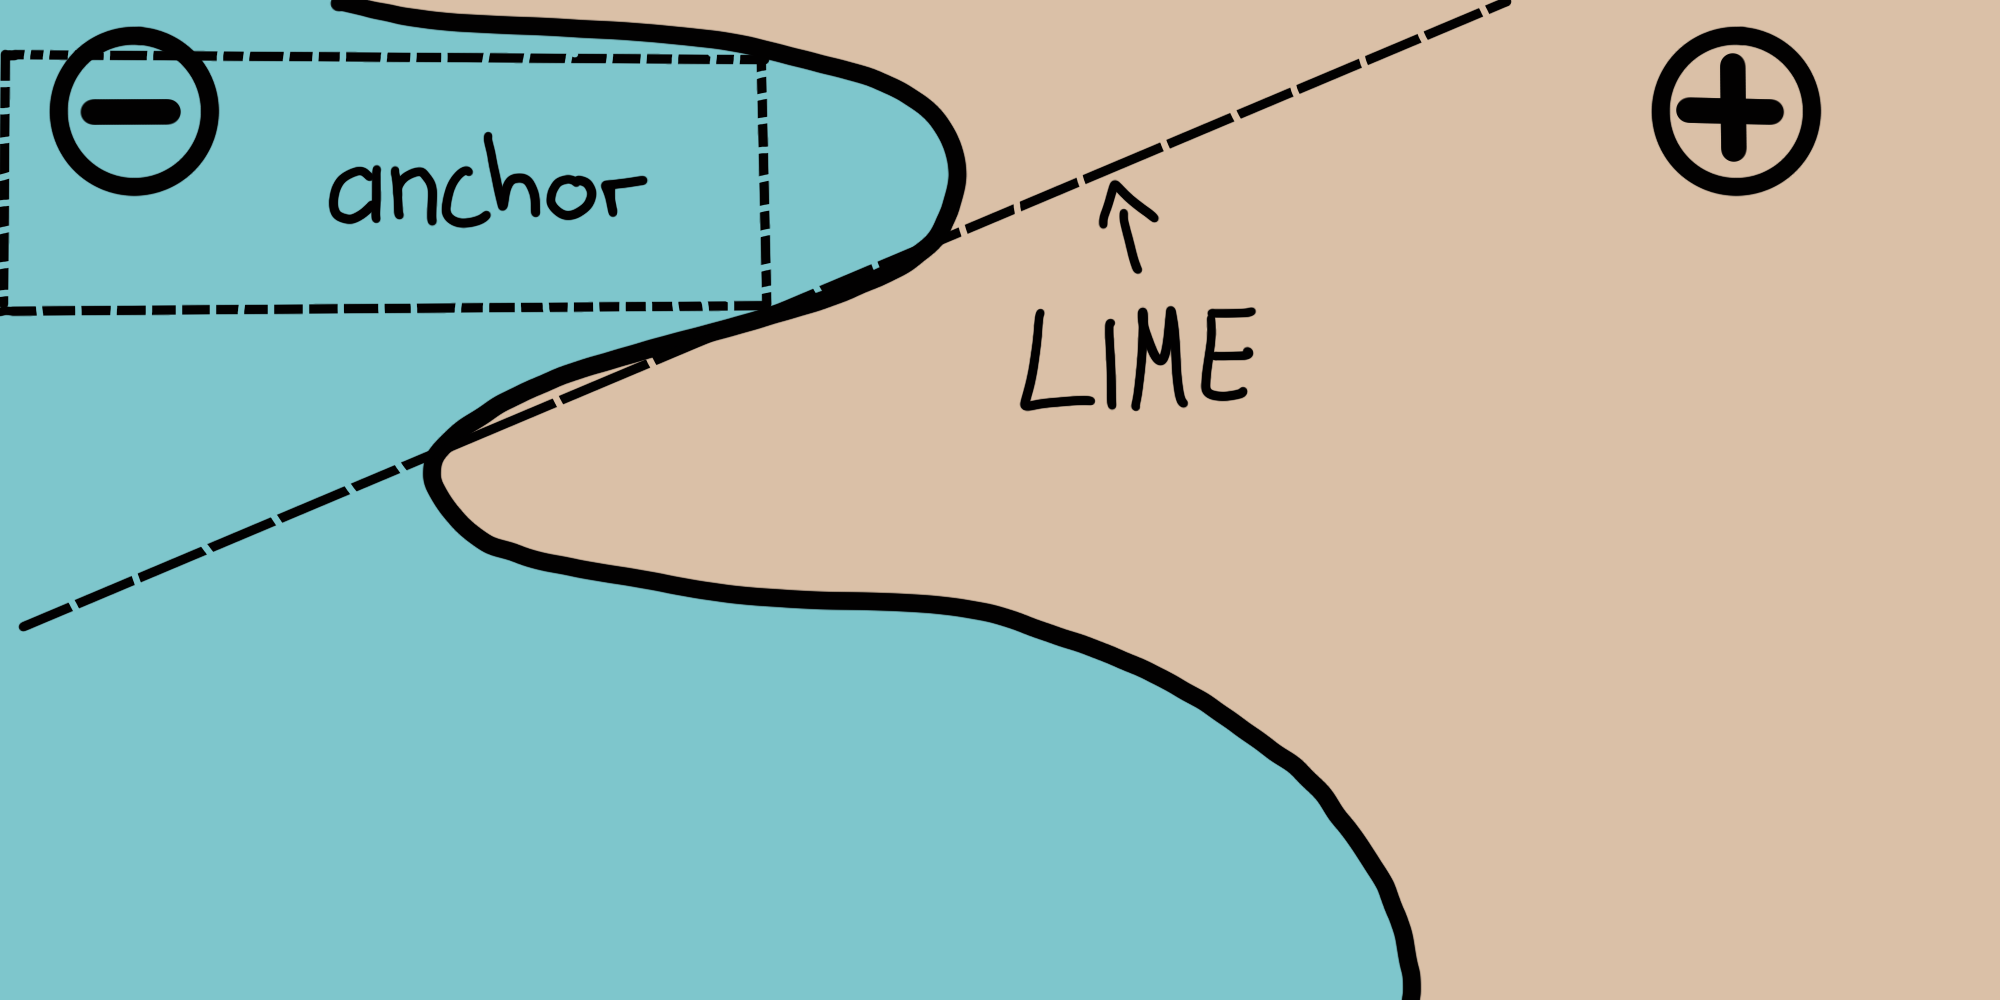
\includegraphics[width=0.85\columnwidth]{Figures/anchors-visualization.png} 
\caption[An example of a floating figure]{LIME vs. Anchors – A Toy Visualization. Figure from Ribeiro, Singh, and Guestrin (2018).} 
\label{fig:LIMEvsANCHORS} 
\end{figure}

%------------------------------------------------

\section{Conclusion}
We saw importance of interpretability in machine learning and then introduced 3 popular methods includes LIME, SHAP, and Anchors which can explain our model.
With help of these methods we can find the points of failure, increase the trust of users in model performance and find the patterns in the data. 

%----------------------------------------------------------------------------------------
%	BIBLIOGRAPHY
%----------------------------------------------------------------------------------------

\printbibliography % Output the bibliography

%----------------------------------------------------------------------------------------

\end{document}
